\documentclass[11pt,oneside,openright]{report} 

\title{Sequence to Sequence learning with a Variational Information Bottleneck}
\author{Tristan Guigue}
\date{2017}

\usepackage[mastersc]{edmaths}
\usepackage[parfill]{parskip}
\usepackage[english]{babel}
\usepackage[utf8]{inputenc}
\usepackage{amsmath}
\usepackage{graphicx}
\usepackage[colorinlistoftodos]{todonotes}
\usepackage{amsmath,amsfonts,amssymb}
\usepackage{float}
\usepackage{tikz}
\usepackage{placeins}
\usepackage{pgfplots}
\usetikzlibrary{bayesnet}
\usepackage[font=small,labelfont=bf]{caption}
\usetikzlibrary{fit, positioning, arrows.meta}
\usepackage[makeroom]{cancel}
\tikzset{
neuron/.style={shape=circle, minimum size=1.1cm,  inner sep=0, draw, font=\small}, io/.style={neuron, fill=gray!20}, deterministic/.style={diamond, minimum size=1.3cm, draw, text badly centered, inner sep=3pt}}
\newtheorem{notation}{Notation}
\newtheorem{definition}{Definition}
\newtheorem{corollary}{Corollary}
\newtheorem{theorem}{Theorem}
\newtheorem{lemma}{Lemma}

\begin{document}

\maketitle

\declaration

\begin{abstract}
TODO
\end{abstract}

\tableofcontents

%------------------------------------------------------------------------------------------------
\chapter{Introduction}

\section{Information Bottlenck Regularisation}
Supervised learning consist in inferring a mapping function between an input and an output from pairs of training example. A good mapping will generalise well to unseen data. If the mapping learned is too complex, the function will be able to map exactly each input to the right output, our training error will be null. However this might not represent the true underlying relationship, we are overfitting. To prevent this, we have to promote simpler mappings using regularisation techniques such as the information bottleneck. 

The idea of the information bottleneck regularisation method introduced by Tishby et al. \cite{tishby}. is to pass the input through an information bottleneck such as to keep only the information that the input contains about the output. In this way we ensure that our mapping won't be affected by noise coming from the input and will reflect what needs to be learn about the input to predict the output. The is especially valid when dealing with high dimensional inputs that contain a lot of information not all relevant to the task.

\section{Motivations}
In sequence to sequence learning we try to map an input sequence to an output sequence. This type of problem can be solved using a encoder to find a representation of the input sequence and a decoder to generate the output sequence. In this case the representation of the input sequence has to contain all the information required to generate the output sequence, this makes it a good candidate to apply the information bottleneck method.

As the information bottleneck method does not have a solution for most inputs we will need to use variational approximations to find a lower bound on our objective and optimise that lower bound as recently shown by Alemi et al. \cite{vib}.
 
\section{Objectives}
In this dissertation we would like to verify that using the information bottleneck regularisation does help getting better performance on sequence to sequence problems. To be able to deal with sequences we would like to use recurrent neural networks as our encoder and decoder. We would like to compare the effect of changing our regularisation parameter and analyse how this affects the learning process.

In particular we would like to apply this model to various setup such as predicting a sequence of pixel to complete an image or finding a list of labels corresponding to a sequence of images.

\section{Structure}

In the second chapter we go through a review of the information bottleneck method, the variational inference framework, introduce recurrent neural networks and the sequence to sequence problem.

In the third chapter we analyse the maximisation of mutual information in different models and compare it to the maximum likelihood to get a better understanding of our model.

In the fourth chapter we present the model we used, derivate the objective function and find a lower bound to optimise. We then find an estimator for this lower bound and explain how to perform gradient descent on the model. Finally we discuss implementation considerations.

In the fifth chapter we explain the experiments that we have setup and present the results in terms of optimal loss or accuracies obtained.

Finally in the conclusion we discuss those results, go through the limitations we encountered and propose further work.

%------------------------------------------------------------------------------------------------
\chapter{Background and Literature Review}
\section{Latent Generative Models and Variational Approximations}
\subsection{Likelihood in Latent Variable Models}
\begin{notation}
Stochastic nodes are represented as circles and deterministic nodes are represented as diamonds. Node of observed data are filled in grey.
\end{notation}

\begin{figure}[H]
\centering
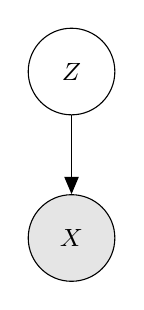
\begin{tikzpicture}[x=2cm, y=1.5cm]
 \node [neuron] (z) {$Z$};
\node [io, below=of z] (x) {$X$};
\draw [->] (z) -- (x);
\end{tikzpicture}
\caption{A simple generative model with a latent variable $Z$}
\end{figure}

A generative model provides assumptions in how observed data was generated. This generation process is assumed to be stochastic in nature, the observed data represented by a random variable $X$ depending stochastically on other random variables. Hidden variables or latents can be introduced to better model the structure believed to have generated the data and include hierarchy. The latents provide compression and representation of the data. They can themselves assumed to be generated by observed variables and be used to predict other variables as we will see in the information bottleneck method. 

We define the likelihood of set of observed data points $x$ under a model with a set of parameters $\theta$ as 
$$\mathcal{L}(\theta|x) = p(x|\theta)$$

For a model with latent variables, those need to be integrated out to find the likelihood:

\begin{equation}
p(x|\theta) = \int p(x|z, \theta) p(z|\theta) dz
\label{eq:lik}
\end{equation}

\subsection{Variational Inference}
\begin{theorem}[Jensen's Inequality]
Let f be a concave function, then
$$ f(\mathbb{E}[x]) \geq \mathbb{E}[f(x)] $$
\end{theorem}

The integral introduced in equation \ref{eq:lik} is intractable in general. To solve this issue we need to approximate the posterior distribution on the latent $p(z|x)$ by a function we can easily sample from and that we call $q_\phi(z|x)$, the parameters $\phi$ of this function are the variational parameters. We can rewrite the integral as:

\begin{align}
p(x|\theta) &= \int p_\theta(x|z) p_\theta(z) \frac{q_\phi(z|x)}{q_\phi(z|x)}dz \\
\end{align}

As the $\log$ is concave we can use Jensen's inequality to find a lower bound for the log likelihood. We note that since the $\log$ is also monotonically increasing finding a maximium for the log likelihood is equivalent to finding a maximum for the likelihood.

\begin{align}
\log p(x|\theta) &= \log \int q_\phi(z|x) p_\theta(x|z) \frac{p_\theta(z)}{q_\phi(z|x)}dz\\
	&\geq  \int q_\phi(z|x) \log \Big[  p_\theta(x|z) \frac{p_\theta(z)}{q_\phi(z|x)} \Big]dz\\
	&=  \mathbb{E}_q[\log  p_\theta(x|z)] - \int q_\phi(z|x) \log   \frac{q_\phi(z|x)}{p_\theta(z)}dz
\label{eq:elbo}
\end{align}

This is the evidence lower bound that can then be optimised by tightening the bound to get as close as possible
to the true marginal likelihood. The solution found is a good approximation to the maximum likelihood if the approximated distribution is close to the true posterior. This way we have turned a problem of integration into one of optimisation. In this dissertation we will use the variational inference principle but apply them to find lower bounds on mutual information rather than likelihood.

\subsection{Sampling}
Another way to overcome the intractability of an expectation is to generate random samples and approximate the results by the mean of those samples. That estimator we get is unbiased.

\subsubsection{Monte Carlo Sampling}
If it is possible to sample directly from the probability $p$ under which we take the expectation then we can use Monte Carlo Sampling.

\begin{theorem}[Law of large numbers]
If $X_i$ is a collection of independent identically distributed random variables with density $p(x)$, then
$$ \lim_{N \to \infty} \frac{1}{N} \sum_i f(X_i) = \int f(x) p(x) dx $$
\end{theorem}

In Monte Carlo sampling we use the law of large number to introduce an estimate  of the expectation:
Let $\theta = \mathbb{E}_{x \sim p(x)}[f(X)]$

Then by the law of large number 

$$ \hat{\theta} =  \frac{1}{N} \sum_i f(X_i) $$ is an unbiased estimate of $\theta$.

\section{The Information Bottleneck}
\subsection{Regularisation in Supervised Learning}
In supervised learning, we try to infer an output given by the random variable $Y$ from an input given by the random variable $X$, learning from labelled training data. The objective is to learn a mapping from $X$ to $Y$ that generalises well to unseen data. To ensure the learning process learns the underlying relationship between $X$ and $Y$ rather than noise in the training data, there are different regularisation techniques possible. We assume here that $Y$ is not independent from the input $X$.

One form of regularisation was introduced by Tishby et al. \cite{tishby}. For each input they seek a stochastic mapping to a representation of the input that provides the most relevant information about the output. They used the concept of mutual information to formalise what a good representation of the input should be extracted. 

The objective is then to learn a representation $Z$ that is maximally compressive on $X$ while being maximally informative about the target $Y$. We want to squeeze the information that $X$ contains about $Y$ trough a bottleneck and keep only the most meaningful information about the output. For example when learning the transcript of words from acoustic data, it is possible to greatly compress the input data while still keeping what is needed to predict the words as the transcript as a much smaller entropy than the acoustic data.

\subsection{Mutual Information}

\begin{definition}
The amount of information that $Z$ contains about $Y$ is given by:
$$ I(Z, Y) = \int p(y, z) \log \frac{p(z, y)}{p(z)p(y)} dy\,dz $$ where Y and Z are continous random variables or 
 $$ I(Z, Y) = \sum_y \sum_z p(y, z) \log \frac{p(z, y)}{p(z)p(y)} $$ where Y and Z are discrete random variables 
\end{definition}

\begin{definition}
The KL divergence from a continuous probability distribution $p$ to another continuous probability distribution $q$ is defined as 
$$ KL[p(x)|q(x)] = \int p(x) \log \frac{p(x)}{q(x)} dx $$
\end{definition}

\begin{corollary}
The mutual information of two random variable is equal to the Kullback-Leibler divergence from the joint distribution of the random variables to the product of the distributions.
$$ I(Z, Y) = KL[p(z, y) | p(z)p(y)] $$
\end{corollary}
The mutual information therefore measures how the joint distribution differs from the product of the marginal distributions. 

\begin{definition}
The entropy of a continuous random variable $Y$ is given by:
$$ H(Y)  = -\int p(y) \log p(y) dy $$
\end{definition}

\begin{definition}
The conditional entropy of a continuous random variable $Y$ given another continuous random variable $Z$ is given by:
$$ H(Y|Z)  = -\int p(y, z) \log p(y|z) dy\,dz $$
\end{definition}
Which can be understood as the how much $Y$ varies when $Z$ is fixed

\begin{corollary}
Let $Y$ and $Z$ be random variables:
\begin{equation}
I(Z, Y) = H(Y) - H(Y|Z)
\label{eq:mutual_info_cond_entropy}
\end{equation}
\end{corollary}

\begin{proof}
\begin{align}
I(Z, Y) &= \int p(y, z) \log \frac{p(z, y)}{p(z)p(y)} dy\,dz\\
& = \int p(y, z) \log \frac{p(y|z)}{p(y)} dy\,dz \label{eq:mi_zy}\\
&= \int p(y, z) \log p(y|z) dy\,dz - \int p(y, z) \log p(y) dy\,dz\\ 
&= - H(Y|Z) - \int p(y) \log p(y) dy\\ 
&= H(Y) - H(Y|Z)
\end{align}
\end{proof}

When $Y$ and $Z$ are independent then  $H(Y|Z) = H(Y)$ and $I(Z, Y) = 0$. 

If $Y$ is a deterministic function of $Z$ then $H(Y|Z) = 0$ and $I(Z, Y) = H(Y)$. 

\subsection{Graphical Model}

\begin{figure}[H]
\centering
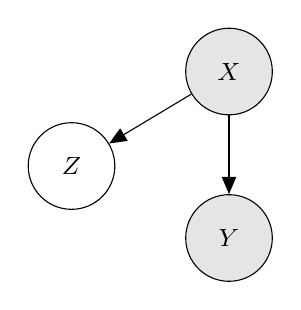
\begin{tikzpicture}[x=2cm, y=1.5cm]
 \node [io] (x) {$X$};
\node [neuron] at (-1, -0.8) (z) {$Z$};
\node [io, below=of x] (y) {$Y$};
\draw [->] (x) -- (z);
\draw [->] (x) -- (y);
\end{tikzpicture}
\caption{Graphical model of the information bottleneck}
\end{figure}

In the information bottleneck model, both the output and the representation depends solely on the input, that is we assume $p(z | x, y) = p(z|x)$. $Z$ is not part of the generative process of $Y$ as it would if $Z$ would be considered a stochastic layer between $X$ and $Y$. In this case $Z$ is only there to ensure we learn a useful representation of $X$ that will help us to predict $Y$.

The factorisation theorem lets us express the joint distribution as:
$$ p(x, y, z) = p(x)\, p(y|x)\, p(z|x)$$

\subsection{Objective function}
In this section we will assume that the random variables are continuous. We define $p_\theta(z|x)$ as our stochastic encoding of the input where $\theta$ are the model parameters. The mutual information of the representation $Z$ and the target $Y$ can then be expressed as:

$$ I(Z, Y|\theta) = \int p_\theta(y, z) \log \frac{p_\theta(z, y)}{p_\theta(z)p(y)} dy\,dz $$

The objective of the information bottleneck method is to maximise $I(Z, Y|\theta)$ while constraining how much information is shared between $X$ and $Z$ such as to force $Z$ to "forget" $X$ and act as a minimal sufficient statistic of $X$ for predicting $Y$. The quantity we are constraining is therefore the mutual information of the input $X$ and its representation $Z$:

$$ I(X, Z|\theta) = \int p_\theta(x, z) \log \frac{p_\theta(x, z)}{p(x)p_\theta(z)} dy\,dz $$

We set $$I(X, Z) < I_c$$ where $I_c$ is the information constraint. This constraint can be expressed using a Lagrange multiplier such as to write the whole objective function as:

$$ J_{IB}(\theta) = I(Z, Y|\theta) - \beta I(X, Z|\theta)$$


\subsection{Iterative Solution}
\begin{theorem}
The information bottleneck objective function has an exact formal solution when X, Y and Z are all discrete:
$$ p(z|x) = \frac{p(z)}{Z(x, \beta)} \exp\Big[-\beta \sum_y p(y|x) \log\frac{p(y|x)}{y|z}\Big] $$
\end{theorem}

The proof can be found in \cite{tishby}. The expression $p(y|z)$ can be expressed as 
 
 \begin{align}
p(y|z) &= \sum_x p(y, x|z)  \\
	 & = \sum_x \frac{p(x ,y, z)}{p(z)} \\
	 &= \frac{1}{p(z)} \sum_x p(x) p(y|x) p (z|x) 
\label{eq:y_given_z}
\end{align}

And $p(z)$ can be expressed as a mixture:
 
  \begin{align}
p(z) &= \sum_x p(z, x)  \\
	 &= \sum_x p(x) p(z|x)
\label{eq:z_post}
\end{align}

In the formal solution, the encoder is present on both sides, Tishby et al. present a scheme to find a optimum by iteratively updating $p(z|x)$, $p(y|z)$ and $p(z)$.

\section{Recurrent Neural Networks}

\subsection{Architecture}
A neural network is a composition of linear and non-linear transformations organised in layers. It is a deterministic function of the input. The output of the neural network is given by:

$$ \hat{y} = f(x | W) = \sigma_L (W_L h_{L-1}(x)) $$

Where:
\begin{itemize}
\item $\hat{y}$ is the predicted output
\item $\sigma$ is a non-linear function
\item $W$ is the set of weights of the linear transformations
\item $L$ is the index of the output layer
\item $h_l$ are the hidden layers defined as:
  \begin{equation}
    \begin{cases}
          h_1(x) = \sigma_1(W_1 x)\\
          h_l(x) = \sigma_l (W_l h_{l-1}(x)) \quad \forall l \in \{2, L\}\\
    \end{cases}
  \end{equation}
\end{itemize}

\begin{figure}[H]
\centering
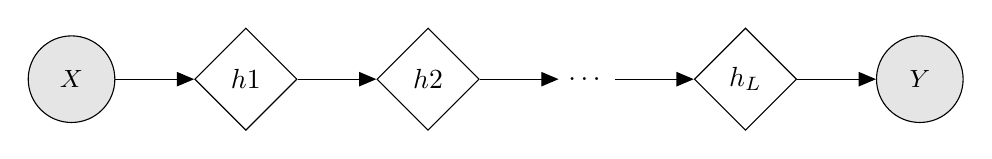
\begin{tikzpicture}[x=2cm, y=1.5cm]
 \node [io] (x) {$X$};
\node [deterministic, right=of x] (h1) {$h1$};
\node [deterministic, right=of h1] (h2) {$h2$};
\node [right=of h2](dots) {\ldots};
\node [deterministic, right=of dots] (hL) {$h_L$};
 \node [io, right=of hL] (y) {$Y$};
\draw [->] (x) -- (h1);
\draw [->] (h1) -- (h2);
\draw [->] (h2) -- (dots);
\draw [->] (dots) -- (hL);
\draw [->] (hL) -- (y);
\end{tikzpicture}
\caption{Graphical model of a neural network}
\end{figure}

In a recurrent neural network as introduced by Graves et al \cite{graves}, an input is given at each time step so the data is processed sequentially, this is especially useful to model language, music, stock prices, etc.

In that case the hidden states at each layer are a linear combination of the input and the previous hidden state such as to carry information from the past:
  \begin{equation}
    \begin{cases}
          h_1(x_1) = \sigma_1(W x_1) \\
          h_l(x_{1:l}) = \sigma_l (U h_{l-1}(x_{1:l-1}) + W x_l) \quad \forall l \in \{2, L\}\\
    \end{cases}
  \end{equation}

We use the same set of weights: U, W at each step since we are performing the same task with different inputs, this makes the parameter space much smaller.

\subsection{Supervised learning settings}
When dealing with sequential data, there are several possible supervised learning problems:
\subsubsection{Many to many}
\begin{figure}[H]
\centering
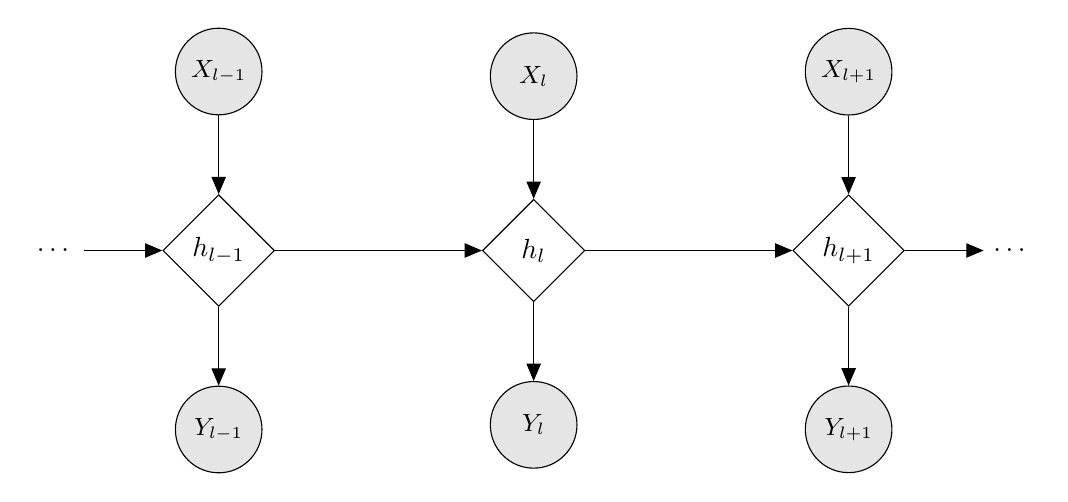
\begin{tikzpicture}[x=2cm, y=1.5cm]
\foreach \jlabel [count=\j, evaluate={\jj=int(\j-1); \jd=int(2 * \j);}]  in {l-1,  l, l+1}{
      \node [deterministic] at (\jd, 1) (h-\j) {$h_{\jlabel}$};
      \node [io, above=of h-\j] (x-\j) {$X_{\jlabel}$};
      \node [io, below=of h-\j] (y-\j) {$Y_{\jlabel}$};
      \draw [->] (x-\j) -- (h-\j);
      \draw [->] (h-\j) -- (y-\j);
      \ifnum\j>1
          \draw [->] (h-\jj.east) -- (h-\j.west);
      \fi
} 
\node [left=of h-1] (ldots){\ldots};
\node [right=of h-3] (rdots){\ldots};
\draw [->] (h-3) -- (rdots);
 \draw [->] (ldots) -- (h-1);
\end{tikzpicture}
\caption{Many to many recurrent neural network graphical model}
\end{figure}
In the many to many problem we try to predict the output at each time step based on previous inputs. For example, we process an image sequentially and try to predict the next pixel at each step, in which case the targets are the next inputs.

In this setting the output is given at each time step by:
$$ \hat{y_l} = f(x_{1:l}|W, U, V) = V h_l(x_{1:l}|W,U)\quad \forall l \in \{1, L\}$$

\subsubsection{Many to one}
\begin{figure}[H]
\centering
\begin{tikzpicture}[x=2cm, y=1.5cm]
\foreach \jlabel [count=\j, evaluate={\jj=int(\j-1); \jd=int(2 * \j);}]  in {1,  2}{
      \node [deterministic] at (\jd, 1) (h-\j) {$h_{\jlabel}$};
      \node [io, above=of h-\j] (x-\j) {$X_{\jlabel}$};
      \draw [->] (x-\j) -- (h-\j);
      \ifnum\j>1
          \draw [->] (h-\jj.east) -- (h-\j.west);
      \fi
} 
\node [right=of h-2] (rdots){\ldots};
\draw [->] (h-2) -- (rdots);
\node [io, above=of h-3] (x-3) {$X_L$};
\node [deterministic, right=of rdots] (h-L) {$h_L$};
\draw [->] (rdots) -- (h-3);
\draw [->] (x-3) -- (h-3);
\node [io, below=of h-3] (y) {$Y$};
\draw [->] (h-L) -- (y);
\end{tikzpicture}
\caption{Many to one recurrent neural network graphical model }
\end{figure}

In the many to one problem, we try to predict the output after having processed a whole sequence. For example we try to predict the label of an image after sequentially processing all the pixels in the image.

In this case the predicted output is given by:
$$ \hat{y} = f(x_{1:L}|W, U, V) = V h_L(x_{1:L}|W,U)$$

\subsubsection{Sequence to sequence}

Sequence to sequence learning aims at predicting an output sequence from an input sequence. Using neural network to solve this was first used by Sutskever et. al. \cite{s2s}. Translation of a sentence is an example of a sequence to sequence task. The output sequence does not necessarily have the same length as the input sequence.


\begin{figure}[H]
\centering
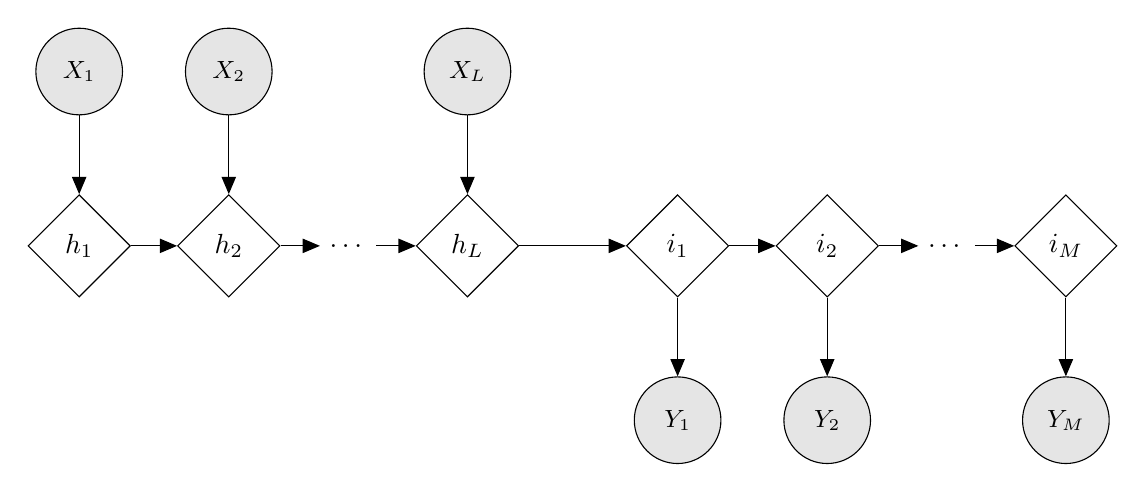
\begin{tikzpicture}[x=0.95cm, y=0.6cm]
\foreach \jlabel [count=\j, evaluate={\jj=int(\j-1); \jd=int(2 * \j);}]  in {1,  2}{
      \node [deterministic] at (\jd, 1) (h-\j) {$h_{\jlabel}$};
      \node [io, above=of h-\j] (x-\j) {$X_{\jlabel}$};
      \draw [->] (x-\j) -- (h-\j);
      \ifnum\j>1
          \draw [->] (h-\jj.east) -- (h-\j.west);
      \fi
} 
\node [right=0.5cm of h-2] (rdots){\ldots};
\draw [->] (h-2) -- (rdots);
\node [deterministic, right=0.5cm of rdots] (h-L) {$h_L$};
\node [io, above=of h-L] (x-L) {$X_L$};
\draw [->] (rdots) -- (h-L);
\draw [->] (x-L) -- (h-L);

\foreach \jlabel [count=\j, evaluate={\jj=int(\j-1); \jd=int(2 * \j);}]  in {1, 2}{
      \node [deterministic] at (8 + \jd, 1) (hpred-\j) {$i_{\jlabel}$};
      \node [io, below=of hpred-\j] (ypred-\j) {$Y_{\jlabel}$};
      \draw [->] (hpred-\j) -- (ypred-\j);
      \ifnum\j>1
          \draw [->] (hpred-\jj.east) -- (hpred-\j.west);
      \fi
} 
\draw [->] (h-L) -- (hpred-1);
\node [right=0.5cm of hpred-2] (rdots){\ldots};
\draw [->] (hpred-2) -- (rdots);
\node [deterministic, right=0.5cm of rdots] (hpred-M) {$i_M$};
\node [io, below=of hpred-M] (ypred-M) {$Y_M$};
\draw [->] (rdots) -- (hpred-M);
\draw [->] (hpred-M) -- (ypred-M);
\end{tikzpicture}
\caption{Sequence to sequence graphical model}
\end{figure}

The output predicting are given with respect to the decoder hidden states:
\begin{equation}
          \hat{y}_{m} = V i_{m} \quad \forall m \in \{1, M\}\\
\end{equation}

\section{Optimisation}
We introduce a loss function using the predicted output and the true values that we intend to minimise.

$$L(x, y, W) = \sum_i l(y_i, \hat{y_i} = f(x_i|W))$$

Where $\{(x_i, y_i)\}$ is our training data. 

In this dissertation we will use the L2 loss for real-valued data:

$$ L(\hat{y}, y) = \lVert \hat{y} - y \rVert^2 $$

Or a cross-entropy loss for binary data:

$$ L(\hat{y}, y) = y \log \hat{y} + (1-y) \log(1 - \hat{y}) $$

\subsection{Gradient Descent}
In most cases a close-form solution to minimising L is not available so we use gradient descent to improve the parameters iteratively.

For a given parameter $w$:

$$ w_{k+1} = w_{k} - \eta \nabla L(x, y, w)$$

We can show that this always decreases $L$ if $\eta$ is small enough. By the first order Taylor expansion:

$$L(w_{k+1}) \approx L(w_{k}) + (w_{k+1} - w_{k})^T  \nabla L_{w}(w_{k}) $$

We get:

$$L(w_{k+1}) \approx L(w_{k}) - \eta | \nabla L(w_{k})|^2 $$

We can iterate this procedure until we reach convergence. However using gradient descent can get us stuck into local optima or saddle points. In this dissertation we use the Adam optimiser \cite{adam} that uses and exponential moving average of the first and second moments of the gradients to improve the optimisation.

 \subsection{Backpropagation}
To obtain the gradient with respect to each parameter $W_l$ in a neural network we use the chain rule to backpropagate the error through the network layers.
 
 \begin{align}
   \nabla_{W_l} L(y, x, W) &= \frac{\partial L}{\partial h_{L-1}} \nabla_{W_l} h_{L-1}\\
   &= \frac{\partial L}{\partial h_{L-1}} \frac{\partial h_{L-1}}{\partial h_{L-2}} \nabla_{W_l} h_{L-2}\\
   &...\\
   &= \frac{\partial L}{\partial h_{L-1}} \frac{\partial h_{L-1}}{\partial h_{L-2}} ... \frac{\partial h_l}{\partial W_l}
 \end{align}
 This is a special case of the reverse mode automatic differenciation and can be done in a computational effective way by storing the required gradients.

\subsection{Vanishing and Exploding Gradients}
In the recurrent neural network setting, our network can be very deep as every input adds a layer to the network. To adjust the weights based on the first input, the error signal is backpropagated from the loss layer all the way to the first layer: 

 \begin{align}
   \nabla_{W_1} L(y, x, W) = \frac{\partial L}{\partial h_{L-1}} \frac{\partial h_{L-1}}{\partial h_{L-2}} ... \frac{\partial h_1}{\partial W_1}
 \end{align}
 
 If we ignore the non-linearity we have:
 $$ \frac{\partial h_{l}}{\partial h_{l-1}} = U $$
 
 And 
 
 $$ \nabla_{W_1} L(y, x, W) = U^{L-1}$$
 
 If we take the univariate example having $u$ smaller than 1 would give a very small gradient, therefore the changes in the parameters of the first layer would be very small and we would have difficulty learning. Vice-versa if $u$ is larger than 1, the gradient will be very large and this will lead to instabilities that will prevent learning the optimal weights. In the multivariate case the gradient will explode if the largest eigenvalue of W is larger than 1, and vanish if the largest eigenvalue is smaller than 1.

\subsection{Gated Recurrent Unit}
To overcome the vanishing or exploding gradient problem, different architecture were proposed including the Gated Recurrent Unit \cite{gru}. Instead of taking $h_l = \sigma(U h_l + W x_l)$ at each step they introduce a gate mechanism that allows a better control of the information that flows through the graph.

The operation performed at each step are the following:
\begin{align}
z_t &= \sigma_g(W_{z} x_t + U_{z} h_{t-1} + b_z) \\
r_t &= \sigma_g(W_{r} x_t + U_{r} h_{t-1} + b_r) \\
h_t &=  z_t \circ h_{t-1} + (1-z_t) \circ \sigma_h(W_{h} x_t + U_{h} (r_t \circ h_{t-1}) + b_h)
\end{align}
Where:
\begin{itemize}
 \item $z_t$ is the update gate that defines how much of the previous memory we keep
 \item $r_t$ is the reset gate that determines how to combine the new input with the previous memory state
\item  $\sigma_g$ is the sigmoid function
\item $\sigma_h$ is a hyperbolic tangent
\end{itemize}

One of the main advantage is that by simply setting the update gate to 1, one can learn the identity. This makes it easier to preserve information from the past.

%------------------------------------------------------------------------------------------------
\chapter{Comparison of Supervised Learning Model}

In this chapter we study the relationship between mutual information maximisation and maximum likelihood in different models.

\section{Fully observed model}

We consider the graphical model of a supervised learning problem where the input is given by the random variable $X$ and the output by the random variable $Y$:

\begin{figure}[H]
\centering
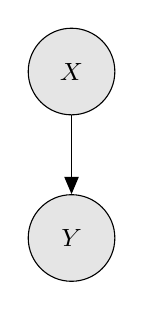
\begin{tikzpicture}[x=2cm, y=1.5cm]
 \node [io] (x) {$X$};
\node [io, below=of x] (y) {$Y$};
\draw [->] (x) -- (y);
\end{tikzpicture}
\end{figure}

We define $p(y|x, \theta)$ as the distribution of the output given the input and our model parameters $\theta$.

The mutual information of $X$ and $Y$ is given by \ref{eq:mutual_info_cond_entropy}:

\begin{align}
I(X, Y) &= H(Y) - H(Y|X)
\end{align}

The entropy of the labels $H(Y)$ is indepedent of our model parameters $\theta$ and will therefore be ignored when taking the gradient with respect to the parameters:

$$ \nabla_\theta I(X,Y) = -\nabla_\theta H(Y|X)$$ 

Using the empirical joint distribution 

$$p(x, y) \approx \frac{1}{N}\sum_n\delta_{x_n}(x)\delta_{y_n}(y)$$

We can approximate the conditional entropy:

\begin{align}
- H(Y|X) &= \int p(x, y) \log p_\theta(y|x) dx\, dy\\
	      &\approx \int \frac{1}{N}\sum_n\delta_{x_n}(x)\delta_{y_n}(y) \log p_\theta(y|x)dx\, dy\\
	      &= \frac{1}{N} \sum_n \log p_\theta(y_n|x_n,)
\end{align}

The log likelihood is given by:
\begin{align}
 l[p_\theta(y|x)] &= \log \prod_n p_\theta(y_n|x_n)\\
 	      &= \sum_n \log p_\theta(y_n|x_n)
\end{align}

We can conclude that mutual information maximisation under an empirical distribution is equivalent to maximum likelihood in this fully observed supervised model:

\begin{align}
\nabla_\theta I(X,Y) = 0 \Leftrightarrow \nabla_\theta l[p_\theta(y|x)] = 0
\end{align}

\section{Stochastic Feed-forward Network}

We now consider a stochastic feed-forward network model that contains an encoder $p_\theta(z|x)$ and a decoder $p_\theta(y|z)$. This is different from the information bottleneck setting as in this case $Z$ is a latent variable part of the generative process of the outputs rather than a representation of the input. This can be useful to introduce depth in the generating process and add stochasticity in a neural network. 

\begin{figure}[H]
\centering
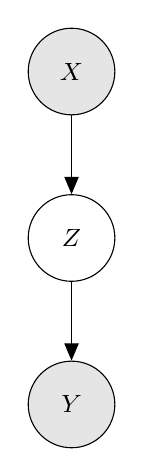
\begin{tikzpicture}[x=2cm, y=1.5cm]
 \node [io] (x) {$X$};
\node [neuron, below=of x] (z) {$Z$};
\node [io, below=of z] (y) {$Y$};
\draw [->] (x) -- (z);
\draw [->] (z) -- (y);
\end{tikzpicture}
\end{figure}

\subsection{Maximum Likelihood}

To get the maximum likelihood we can simply use a Monte Carlo approximation to the expectation of the decoder under the encoder distribution:

\begin{align}
 p(y|x) &= \int p_\theta(y, z|x) dz \\
 &= \int p_\theta(y|z) p_\theta(z|x) dz \\
 &= E_{Z | X}[p_\theta(y|z)] 
\end{align}

Which becomes:
\begin{align}
 p_\theta(y|x) &\approx \frac{1}{M} \sum^M_{m=1} p(y | z^{(m)}) 
\end{align}

Where $ z^{(m)} \sim p_\theta(z|x) $

However this estimator have a high variance in high dimensional space because our draw from $p_\theta(z | x)$ might not contribute significantly to our estimate $p(y |x)$. For most $z$, $p_\theta(y|z)$ will be nearly zero. We would need an very large number of samples to ensure we will generate samples that contribute to $p(y|x)$, this makes it impractical.

\subsubsection{Stochastic Gradient Variational Bayes}

To solve this, we would like to sample values of $Z$ that are likely to have produced $Y$. To do so we introduce a variational approximation $q_\phi(z|x, y)$ of $p(z|x, y)$ and optimise the variational lower bound with respect to the variational parameters $\phi$.
 
\begin{align}
 \log p(y|x) &= \log(\int p_\theta(y, z|x) dz) \\
 & =  \log(\int q_\phi(z|x, y) \frac{p_\theta(y, z|x)}{q_\phi(z|x, y)}) \\
 & \geq \int q_\phi(z|x, y) \log \frac{p_\theta(y, z|x)}{q_\phi(z|x, y)}
\end{align}

Using Jensen's inequality.

\begin{align}
 \log p(y|x) & \geq \int q_\phi(z|x, y) \log \frac{p_\theta(z|x) p_\theta(y| z)}{q_\phi(z|x, y)} \\
  &= \int q_\phi(z|x, y) \log \frac{p_\theta(z|x)}{q_\phi(z|x, y)}  + \int q_\phi(z|x, y) \log p_\theta(y|z) \\
  &= E_q[p_\theta(y|z)] - KL\big[q_\phi(z|x, y) || p_\theta(z|x)]\\
  &\approx  \frac{1}{M} \sum^M_{m=1} p_\theta(y | z^{(m)}) - KL\big[q_\phi(z|x, y) || p_\theta(z|x)\big]
\end{align}
Where $ z^{(m)} \sim q_\phi(z|x, y)$, using a Monte Carlo approximation of the expectation and assuming the KL divergence can be computed analytically.

The bound is exact when $q_\phi(z| x, y) = p(z|x, y)$. The first term corresponds to the reconstruction cost and the KL divergence between $q_\phi(z|x, y)$ and $p_\theta(z|x)$ acts as a regulariser. 

\subsection{Maximum Mutual Information}

We would like to compare this result to the maximisation of the  mutual information between Z and Y:

\begin{align}
I(Z, Y|\theta) &= \int p_\theta(y, z) \log \frac{p_\theta(z, y)}{p_\theta(z)p(y)} dy\,dz\\
& = \int p_\theta(y, z) \log \frac{p_\theta(y|z)}{p(y)} dy\,dz\\
&= \int p_\theta(y, z) \log p_\theta(y|z) dy\,dz - H(Y) 
\end{align}
We ignore the entropy of the labels as it is independent of our model parameters. We get:
\begin{align}
I(Z, Y|\theta) &= \int p_\theta(x, y, z) \log p_\theta(y| z) dx\,dy\,dz + C\\
&= \int p_\theta(z | x, y) p(x, y) \log p_\theta(y | z) dx\,dy\,dz + C
\end{align}
We can approximate the empirical joint distribution of the data and the labels:
$$ p(x, y) \approx \frac{1}{N}\sum_n \delta_{x_n}(x) \delta_{y_n}(y)$$
And we get:
$$ I(Z, Y|\theta) \approx \frac{1}{N} \int p(z | x^{(n)}, y^{(n}) \log p_\theta(y^{(n)} | z) + C$$

As we can see this is not equivalent to the maximum likelihood results. In particular we have no way to easily get the posterior over z. 

%------------------------------------------------------------------------------------------------
\chapter{Model}
\section{Deep Variational Information Bottleneck}

In the first chapter a solution to the information bottleneck problem was presented when X, Y and Z are all discrete. However in the general case there won't be a formal solution or an iterative method to find the parametric encoder. Alemi at al. in \cite{vib} introduce a variational approach to the information bottleneck. They use variational inference to provide a lower bound to the information bottleneck objective. This allow us to use stochastic gradient ascent to find an optimum of the lower bound and to parametrise the encoder with a neural network which can handle a broad range of data.

\subsection{Variational Lower Bound}

\subsubsection{Lower bound on $I(Z, Y)$}
The equation \ref{eq:y_given_z} is not tractable in the continuous case. Indeed
\begin{align}
p_\theta(y|z) &= \frac{1}{p(z)} \int p(x, y) p_\theta(z|x) dx
\end{align}

Using $q_\phi(y|z)$ as a variational approximation to $p(y|z)$ we can find a lower bound to the mutual information of $Y$ and $Z$ as proposed in Barber et al. \cite{barber}.

\begin{lemma}
A lower bound to the mutual information of $Y$ and $Z$ is:
$$ \mathcal{L}^{A}(x, y, \theta, \phi) = \int p(x)\, p(y|x)\, p_\theta(z|x) \log q_\phi(y|z) dy\, dz\, dx + H(Y)$$
\end{lemma}

\begin{proof} In \ref{appendix:xz}\end{proof}
Note that since the entropy of the label is a constant, it will be ignored in our objective function.

If $q_\phi(z|y) = p(z|y)$, the bound is exact. When optimising the lower bound we will increase $I(Z, Y)$ while minimising $KL\big[q_\phi(z|y)|p(z|y)\big]$ which mean our approximation will get closer to the true posterior.

\subsubsection{Upper bound on $I(X, Z)$}
The marginal on $Z$ given in equation \ref{eq:z_post} is intractable as well:

$$ p(z) = \int p_\theta(z|x) p(z) dx $$

We also approximate the marginal on $Z$ $p(z)$ by $r_\psi(z)$ which gives us the second part of the objective function. 

\begin{lemma}
An upper bound to the mutual information of $X$ and $Z$ is:
$$ \mathcal{U}(x, y, \theta, \psi) = \int p(x)p(y|x)p_\theta(z|x) \log \frac{p_\theta(z|x)}{r_\psi(z)}dx\, dy\, dz$$
\end{lemma}

\begin{proof} In \ref{appendix:zy}\end{proof}

\begin{theorem}
A lower bound to the information bottleneck objective function can be written as:
 \begin{align}
\mathcal{L}(x, y, \theta, \phi, \psi) = \int p(x) p(y|x) p_\theta(z|x) \Big[ \log q_\phi(y|z) - \beta  \log \frac{p_\theta(z|x)}{r_\psi(z)}\Big] dx\, dy\, dz
\end{align}
\end{theorem}

One possibility to to find an optimum to this problem would be to update iteratively the model parameter $\theta$ from $p_\theta(z|x)$  and the variational parameters $\phi$ and $\psi$ from $q_\phi(y|z)$ and $r_\psi(z)$ in a procedure similar to the variational expectation maximisation algorithm \cite{vem} for the maximum likelihood. Instead we will use a variational bayes inference method to learn together both the model and variational parameters and use stochastic gradient descent to optimise the bound.

We also note that the tightness of the bound depends on both variational approximations made.

\subsection{Estimating the lower bound}
Since X and Y are known during training, we can use the empirical data distribution $\tilde{p}(x, y) = \frac{1}{N}\sum_n\delta_{x_n}(x)\delta_{y_n}(y)$ to approximate the lower bound:

 \begin{align}
\tilde{\mathcal{L}} & = \int \tilde{p}(x, y) p_\theta(z|x) \Big[\log q_\phi(y|z) - \beta \log \frac{p_\theta(z|x)}{r_\psi(z)} \Big]dx\, dy\, dz  \\
   & = \int \frac{1}{N}\sum_n\delta_{x_n}(x)\delta_{y_n}(y) p_\theta(z|x) \Big[\log q_\phi(y|z) - \beta \log \frac{p_\theta(z|x)}{r_\psi(z)} \Big] dx\, dy\, dz \\
   & = \frac{1}{N}\sum_n \int \delta_{x_n}(x)\delta_{y_n}(y) p_\theta(z|x) \Big[ \log q_\phi(y|z) - \beta \log \frac{p_\theta(z|x)}{r_\psi(z)}\Big ] dx\, dy\, dz \\
   & = \frac{1}{N}\sum_n \int p_\theta(z|x_n) \Big[  \log q_\phi(y_n|z_n) - \beta   \log \frac{p_\theta(z|x_n)}{r_\psi(z)} \Big] dz \label{eq:lower}
\end{align}


\subsection{Reparametrisation Trick}
To apply gradient descent we would like to get the gradient with respect to the parameters for the lower bound estimation \ref{eq:lower}. However the first part of the estimator is problematic. Indeed we are taking the gradient of the parameters under which the expectation is taken: $\theta$.

One way to solve this would be using the score function:
 \begin{align}
\nabla_\theta \mathbb{E}_{p_\theta(z|x)}\big[ g(z) \big] &= \int_z \nabla_\theta p_\theta(z|x)  g(z)\\
 &= \int_z \frac{p_\theta(z|x)}{p_\theta(z|x)} \nabla_\theta p_\theta(z|x)  g(z) \\
 &= \int_z p_\theta(z|x) \nabla_\theta \log p_\theta(z|x)  g(z)\\
&= \mathbb{E}_{p_\theta(z|x)}\big[ \nabla_\theta \log p_\theta(z|x) g(z)  \big]\\
&\approx \frac{1}{L} \sum_l  g(z^{(l)}) \nabla_\theta \log p_\theta(z^{(l)}|x)
\end{align}

Where $z^{(l)} \sim p_\theta(z|x)$.

However it has been shown that this gradient estimator exhibits very high variance and is therefore impractical.

\begin{figure}[H]
    \centering
    \begin{minipage}{0.45\textwidth}
        \centering
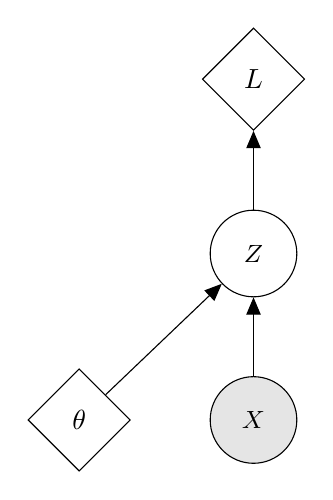
\begin{tikzpicture}[x=2cm, y=1.5cm]
 \node [neuron] (z) {$Z$};
\node [io, below=of z] (x) {$X$};
\node [deterministic, left=of x] (theta) {$\theta$};
\node [deterministic, above=of z] (l) {$L$};
\draw [->] (x) -- (z);
\draw [->] (theta) -- (z);
\draw [->] (z) -- (l);
\end{tikzpicture}
        \caption{Initial Model}
    \end{minipage}\hfill
    \begin{minipage}{0.45\textwidth}
        \centering
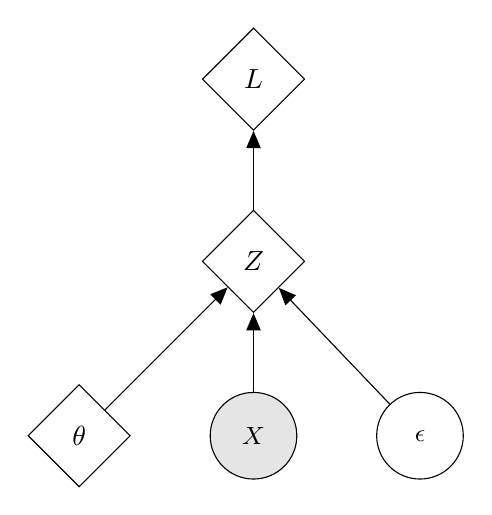
\begin{tikzpicture}[x=2cm, y=1.5cm]
 \node [deterministic] (z) {$Z$};
\node [io, below=of z] (x) {$X$};
\node [deterministic, left=of x] (theta) {$\theta$};
\node [deterministic, above=of z] (l) {$L$};
\node [neuron, right=of x] (eps) {$\epsilon$};
\draw [->] (x) -- (z);
\draw [->] (theta) -- (z);
\draw [->] (z) -- (l);
\draw [->] (eps) -- (z);
\end{tikzpicture}
        \caption{Reparametrised Model}
    \end{minipage}
\end{figure}

Another way to solve this issue is to use the reparametrisation trick also called pathwise estimator  from Kingma \& Welling \cite{kingma} and write $z$ as a deterministic function of the model parameter $\theta$ and a random variable $\epsilon$: $z = f(\theta(x), \epsilon)$. We can then write:
$$p(z) = p(\epsilon) \Big|\frac{d\epsilon}{dz} \Big| \Rightarrow |p(\epsilon) d\epsilon| = |p(z|x) dz|$$
The gradient can then be propagated back to the input and the parameters through the deterministic node $Z$:
\begin{align}
\nabla_\theta \int p_\theta(z|x) g(z) dz &= \nabla_\theta \int p(\epsilon) g\big(f(\theta(x), \epsilon)\big) d\epsilon\\
&= \int p(\epsilon) \nabla_\theta g\big(f(\theta(x), \epsilon)\big) d\epsilon\\
&= \mathbb{E}_{p(\epsilon)}\Big[\nabla_\theta g\big(f(\theta(x), \epsilon)\big)\Big]
\end{align}

We can therefore rewrite the estimator as:

 \begin{align}
\tilde{\mathcal{L}}   &= \frac{1}{N}\sum_n  \mathbb{E}_{\epsilon \sim p(\epsilon)}\Big[  \log q(y_n|f(x_n, \epsilon)) - \beta  \log \frac{p(f(x_n, \epsilon)|x_n)}{r(f(x_n, \epsilon))}\Big]  \label{eq:lower2}
\end{align}

Note that if the the KL divergence can be calculated analytically as it is the case if both distribution are gaussian we can write more simply:

 $$ \tilde{\mathcal{L}}  = \frac{1}{N}  \sum_{n=1}^{N} \mathbb{E}_{\epsilon \sim p(\epsilon)}\Big[\log q(y_{n} |f(x_{n}, \epsilon))\Big] - \beta KL[p(Z|x_{n}), r(Z)]$$

To turn this into a minimisation problem, the obective function becomes:

 $$ J_{VIB} = \frac{1}{N}  \sum_{n=1}^{N} \mathbb{E}_{\epsilon \sim p(\epsilon)}\Big[-\log q(y_{n} |f(x_{n}, \epsilon))\Big] + \beta KL\big[p(Z|x_{n}), r(Z)\big]$$


The first part of of the lower bound correspond to the cost of constructing $Y$ under our model from $Z$, that is how well our samples from $p_\theta(z|x)$ explains the data $Y$. The second part is a penalty or regularisation term that correspond to the number of bits we need to construct $Z$.

\section{Application to Sequential Data}

We apply the variational information bottleneck method to find a good representation of a sequence rather than a single input. We will use recurrent neural networks to combine the inputs and pass the last hidden layer of the network through an information bottleneck to get a robust representation of the sequence. As we have seen in the first chapter there are different supervised learning problem for sequential data we will see how to apply the variational information bottleneck in each setting.

\subsection{Many to many}
\begin{figure}[H]
\centering
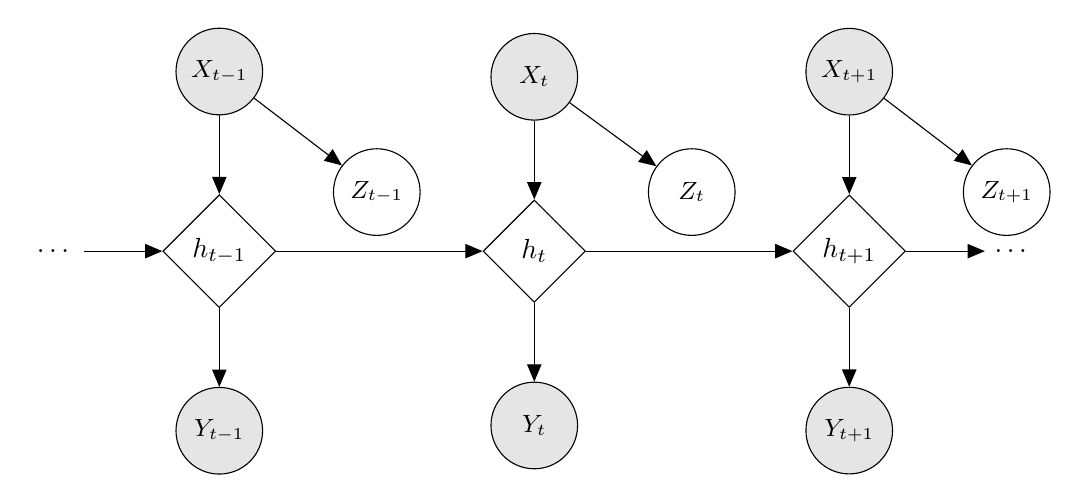
\begin{tikzpicture}[x=2cm, y=1.5cm]
\foreach \jlabel [count=\j, evaluate={\jj=int(\j-1); \jd=int(2 * \j);}]  in {t-1,  t, t+1}{
      \node [deterministic] at (\jd, 1) (h-\j) {$h_{\jlabel}$};
       \node [neuron] at (\jd + 1, 1.5) (z-\j) {$Z_{\jlabel}$};
      \node [io, above=of h-\j] (x-\j) {$X_{\jlabel}$};
      \node [io, below=of h-\j] (y-\j) {$Y_{\jlabel}$};
      \draw [->] (x-\j) -- (h-\j);
      \draw [->] (x-\j) -- (z-\j);
      \draw [->] (h-\j) -- (y-\j);
      \ifnum\j>1
          \draw [->] (h-\jj.east) -- (h-\j.west);
      \fi
} 
\node [left=of h-1](ldots) {\ldots};
\node [right=of h-3](rdots) {\ldots};
\draw [->] (ldots) -- (h-1);
\draw [->] (h-3) -- (rdots);
\end{tikzpicture}
\caption{Graphical model of many to many variational information bottleneck}
\end{figure}

In the many to many problem we try to find at each time step a representation $Z_t$ that is maximally compressive of each input $X_t$ and maximally predictive about future outputs. The objective function can therefore be written as:

$$ J_{IB} = \sum_t I(Z_t, Y_{t}) - \beta I(X_{t}, Z_t)$$
 
 The problem with this setting is that the representation $Z_t$ does not contain information about the past, therefore they won't be good predictor of the outputs. One way to solve this would be to have $Z_t$ depend on all previous inputs. However in that case the $Z_t$ won't be independent and therefore we wouldn't be able to decompose the objective function as we did.
 
\subsection{Many to one}

\begin{figure}[H]
\centering
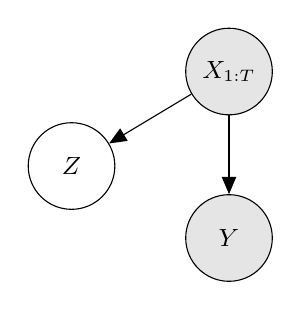
\begin{tikzpicture}[x=2cm, y=1.5cm]
 \node [io] (x) {$X_{1:T}$};
\node [neuron] at (-1, -0.8) (z) {$Z$};
\node [io, below=of x] (y) {$Y$};
\draw [->] (x) -- (z);
\draw [->] (x) -- (y);
\end{tikzpicture}
\caption{Graphical model of many to one variational information bottleneck}
\end{figure}

The many to one problem is similar to the original supervised problem. Indeed we can consider the whole sequence as a random variable and apply the information bottleneck on this. When implementing this we will use the output of a recurrent neural network and pass it through the information bottleneck to get a representation of the sequence that is maximally compressive on the input sequence while being maximally predictive on the output sequence.

\begin{figure}[H]
\centering
\begin{tikzpicture}[x=2cm, y=1.5cm]
\foreach \jlabel [count=\j, evaluate={\jj=int(\j-1); \jd=int(2 * \j);}]  in {1,  2}{
      \node [deterministic] at (\jd, 1) (h-\j) {$h_{\jlabel}$};
      \node [io, above=of h-\j] (x-\j) {$X_{\jlabel}$};
      \draw [->] (x-\j) -- (h-\j);
      \ifnum\j>1
          \draw [->] (h-\jj.east) -- (h-\j.west);
      \fi
} 
\node [right=of h-2] (rdots){\ldots};
\draw [->] (h-2) -- (rdots);
\node [io, above=of h-3] (x-3) {$X_T$};
\node [deterministic, right=of rdots] (h-L) {$h_T$};
\draw [->] (rdots) -- (h-3);
\draw [->] (x-3) -- (h-3);
\node [neuron] at (7, 3.5) (z) {$Z$};
\draw [->] (x-1.north) -- (z);
\draw [->] (x-2.north) -- (z);
\draw [->] (x-3.north) -- (z);
\node [io, right=of h-L] (y) {$Y$};
\draw [->] (h-L) -- (y);
\end{tikzpicture}
\caption{Graphical model of many to one variational information bottleneck }
\end{figure}

When drawing the graphical model we display the hidden states of the generative model rather than the hidden state of the encoder although in practice we will use a recurrent neural network that also contain hidden states to get a representation of the input sequence. Similarly the variational approximation $q_\phi(y|z)$ are not shown in this graphical model as they are not part of the generative process.

The information bottleneck objective is then:
$$ J_{IB} = I(Z, Y) - \beta I(X_{1:T}, Z)$$
Whose lower bound objective under the variational approximation becomes:
 $$ J_{VIB} = \frac{1}{N}  \sum_{n=1}^{N} \mathbb{E}_{\epsilon \sim p(\epsilon)}[- \log q(y^{n} |f(x_{1:T}^n, \epsilon))] + \beta KL[p(Z|x_{1:T}^n), r(Z)]$$

\subsection{Sequence to Sequence}
Sequence to sequence problems have first been used in the context of recurrent neural network by Sutskever \cite{s2s}. They are especially useful for translation. The deterministic model compresses the whole input sequence into a hidden state from which the output sequence is generated. This makes it a good candidate for the information bottleneck framework as pulling a relevant representation out of the input is crucial to be able to generate an accurate output sequence. Recent models have included attention \cite{attention} models or other external memory mechanism to go around this bottleneck ,we will discuss this in the conclusion.

\begin{figure}[H]
\centering
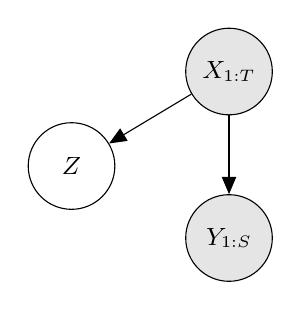
\begin{tikzpicture}[x=2cm, y=1.5cm]
 \node [io] (x) {$X_{1:T}$};
\node [neuron] at (-1, -0.8) (z) {$Z$};
\node [io, below=of x] (y) {$Y_{1:S}$};
\draw [->] (x) -- (z);
\draw [->] (x) -- (y);
\end{tikzpicture}
\caption{Sequence to sequence variational information bottleneck graphical model}
\end{figure}

The graphical model of this problem is also similar to the original information bottleneck graphical model if we consider the input and output sequences as random variables. Representing the hidden states of the graphical model we get: 


\begin{figure}[H]
\centering
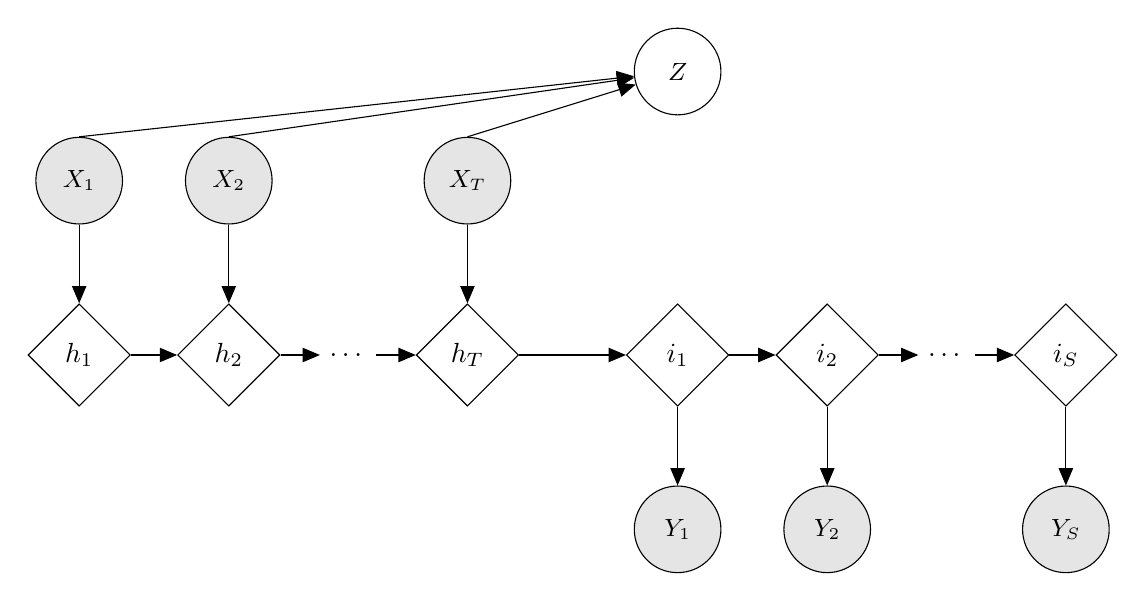
\begin{tikzpicture}[x=0.95cm, y=0.6cm]
\foreach \jlabel [count=\j, evaluate={\jj=int(\j-1); \jd=int(2 * \j);}]  in {1,  2}{
      \node [deterministic] at (\jd, 1) (h-\j) {$h_{\jlabel}$};
      \node [io, above=of h-\j] (x-\j) {$X_{\jlabel}$};
      \draw [->] (x-\j) -- (h-\j);
      \ifnum\j>1
          \draw [->] (h-\jj.east) -- (h-\j.west);
      \fi
} 
\node [right=0.5cm of h-2] (rdots){\ldots};
\draw [->] (h-2) -- (rdots);
\node [deterministic, right=0.5cm of rdots] (h-L) {$h_T$};
\node [io, above=of h-L] (x-L) {$X_T$};
\draw [->] (rdots) -- (h-L);
\draw [->] (x-L) -- (h-L);

\foreach \jlabel [count=\j, evaluate={\jj=int(\j-1); \jd=int(2 * \j);}]  in {1, 2}{
      \node [deterministic] at (8 + \jd, 1) (hpred-\j) {$i_{\jlabel}$};
      \node [io, below=of hpred-\j] (ypred-\j) {$Y_{\jlabel}$};
      \draw [->] (hpred-\j) -- (ypred-\j);
      \ifnum\j>1
          \draw [->] (hpred-\jj.east) -- (hpred-\j.west);
      \fi
} 
\draw [->] (h-L) -- (hpred-1);
\node [right=0.5cm of hpred-2] (rdots){\ldots};
\draw [->] (hpred-2) -- (rdots);
\node [deterministic, right=0.5cm of rdots] (hpred-M) {$i_S$};
\node [io, below=of hpred-M] (ypred-M) {$Y_S$};
\draw [->] (rdots) -- (hpred-M);
\draw [->] (hpred-M) -- (ypred-M);
\node [neuron] at (10, 7) (z) {$Z$};
\draw [->] (x-1.north) -- (z);
\draw [->] (x-2.north) -- (z);
\draw [->] (x-L.north) -- (z);
\end{tikzpicture}
\caption{Sequence to sequence variational information bottleneck graphical model}
\end{figure}


The information bottleneck objective is then:
$$ J_{IB} = I(Z, Y_{1:S}) - \beta I(X_{1:T}, Z)$$
Whose lower bound objective under the variational approximation becomes:
 $$ J_{VIB} = \frac{1}{N}  \sum_{n=1}^{N} \mathbb{E}_{\epsilon \sim p(\epsilon)}[- \log q(y_{1:S}^n |f(x_{1:T}^n, \epsilon))] + \beta KL[p(Z|x_{1:T}^n), r(Z)]$$

\section{Model Implementation}
\subsection{Stochastic encoder $p_\theta(z|x_{1:T})$}
Like in \cite{vib} we choose our encoder to be a gaussian whose mean and variance will be given by the output of a neural network:
$$ p(z|x) \sim \mathcal{N}(z | f^\mu(x_{1:T}), f^\Sigma(x_{1:T}))$$ where $f^\mu$ and $f^\Sigma$ are given by a recurrent neural network.

Since the encoder is a gaussian we can use  $z = f(x, \epsilon) =  \mu(x) + \Sigma(x)^{1/2} \epsilon$ for the reparametrisation trick where $\epsilon \sim \mathcal{N}(0, I)$. 
 
\subsection{Decoder $q_\phi(y|z)$}
For the variational approximation of $p(y|z)$ we use a simple logistic regression:

$$ q_\phi(y|z) \sim \mathcal{C}(y| \mathcal{S}(Wz + b)))$$ where $\mathcal{C}$ is a categorical distribution and $\mathcal{S}$ is the softmax function. Note that we won't actually sample from the categorical distribution we will rather take the expected values for each categories given by the softmax and feed those values to our cross-entropy loss function. This has been shown to work well in practice \cite{draw}.

\subsection{Marginal $r_\psi(z)$}

As an approximation to the marginal we can use as a simple non-parametric approximation:
$$r_\psi(z) \sim \mathcal{N}(0, I)$$

However to improve the expressiveness of the marginal distribution on the latent, we can allow its parameters to be learned. 

$$r_\psi(z) \sim \mathcal{N}(\mu_r, \Sigma_r)$$

In the objective function we calculate the KL divergence from $p_\theta(z|x) \sim \mathcal{N}(\mu_p, \Sigma_p)$ to $r_\psi(z) \sim \mathcal{N}(\mu_r, \Sigma_r)$. Since both are assumed to be gaussians with diagonal variance we can use:

\begin{align}
KL[\mathcal{N}_p| \mathcal{N}_r] &= \frac{1}{2}(Tr(\Sigma_r^{-1}\Sigma_p) + (\mu_r - \mu_p)^T\Sigma_r^{-1}(\mu_p - \mu_r) - k + \log\frac{|\Sigma_r|}{|\Sigma_p|})\\
&= \frac{1}{2}(\sum_i \frac{\Sigma_{p, ii}}{\Sigma_{r, ii}} + \sum_i \frac{(\mu_{r_i} - \mu_{p, i})^2}{\Sigma_{r, ii}} - k + \log\frac{\prod \Sigma_{r, ii}}{\prod \Sigma_{p, ii}})\\
&= \frac{1}{2}(\sum_i[ \log \Sigma_{r, ii} - \log \Sigma_{p, ii} - 1 + \frac{\Sigma_{p, ii}}{\Sigma_{r, ii}} + \frac{(\mu_{r_i} - \mu_{p, i})^2}{\Sigma_{r, ii}}]
\end{align}

In the case where $r_\psi(z)$ is a standard normal prior we get:
\begin{align}
KL[\mathcal{N}_p | \mathcal{N}_0] &= \sum_i[ -\log \Sigma_{p, ii} - 1 + \Sigma_{p, ii}+ \mu_{p, i}^2]
\label{eq:kl}.
\end{align}

\subsection{Monte Carlo Expectation}

In the lower bound we have to take an expectation with respect $p(\epsilon)$. To do so we take S Monte Carlo samples: 
 $$ \mathbb{E}_{\epsilon \sim p(\epsilon)}[- \log q(y_{n} |f(x_{n}, \epsilon))] \approx \frac{1}{S}\sum_s - \log q(y_{n} |f(x_{n}, \epsilon_s)) $$
 
 In practice, we use S = 1 or S = 12. Taking more samples would give a better estimate however since we are using stochastic gradient descent, we are already averaging on the batches and therefore have a doubly stochastic gradient estimator.

\subsection{Computational Graph}
\begin{center}
\includegraphics[scale=0.4]{model}
\captionof{figure}{Computational Graph of the Sequence to Sequence Variational Information Bottleneck. The loss layers are indicated in blue and the stochastic layers in red.}
\end{center}

\paragraph{Input Sequence}
The input sequence is passed through a recurrent neural network consisting of GRU cells. The output of the last layer is then pass to the stochastic encoder.

\paragraph{Stochastic Encoder}
The encoder takes as input the output of the last layer of the recurrent neural network. We apply a linear transformation to get a vector of twice the size of the bottleneck. The output is then split in two, the first part is used to get the mean of the gaussian distribution and the second part to get the diagonal terms of the covariance matrix after passing through a softplus function. The covariance is chosen to be diagonal for computational efficiency, as a consequence the features represented by $Z$ cannot be correlated. The encoding $z$ is then found by applying the reparametrisation trick transformation to a sample $\epsilon$ from the standard normal.

\paragraph{Decoder}
A linear transformation is applied to the encoding $z$  to get an vector of the size of the hidden layer of the decoding RNN. The decoding RNN uses this vector as an initial state provides an output at each step. Those output are linearly transformed to get a vector of the size of the number of labels. 

\paragraph{Loss}
The KL divergence is calculated from the encoder mean and variance and compared to the standard normal using equation \ref{eq:kl}. The reconstruction cost is calculated using a cross-entropy loss between the true label and the probabilities given by the decoder.

\subsection{Architecture Details }
\paragraph{Exponential Moving Average}
To get more stable test results we keep track of the exponential moving average of the parameter values during training and use those at test time. The average values are defined as

$$w_{avg}^{k+1} = \tau w_{avg}^k  + (1 - \tau) w^k$$

Where $\tau$ is the decay constant that we took as 0.999.

\paragraph{Software Implementation}
We use TensorFlow to implement our models and run them on a single GPU. We use stochastic gradient descent to optimise our loss function with a batch size of 100 and a learning rate of $10^{-4}$.

%------------------------------------------------------------------------------------------------
\chapter{Experiments and Results}
\section{One to one}
\subsection{MNIST image to label}

In this experiment we try to predict the label of a hand-written digit MNIST \cite{mnist} image.  We use the same parameters as in the Deep Variational Information Bottleneck paper \cite{vib}, the objective is to verify that we could reproduce similar results and that the information bottleneck method is indeed effective in a simple setup.

\begin{minipage}{0.35\textwidth}
        \centering
\begin{tabular}{ c | c  }
 Hidden units & 1024 \\
 Bottleneck size & 256 \\
\end{tabular}
\captionof{figure}{Parameters}
    \end{minipage}\hfill
    \begin{minipage}{0.8\textwidth}
        \centering
\begin{tabular}{ c | c c }
 $\beta$ & accuracy & loss \\
 \hline
0 & 98.48 & 0.058 \\
$10^{-7}$ & 98.58 & 0.057\\
$10^{-6}$ & 98.55 & 0.060\\
$10^{-5}$ & 98.67 & 0.058\\
$10^{-4}$ & 98.71 & 0.053 \\
$10^{-3}$ & 98.68 & 0.059 \\
$10^{-2}$ & 98.42 & 0.095 \\
\end{tabular}
\captionof{figure}{Results}
    \end{minipage}

\begin{center}
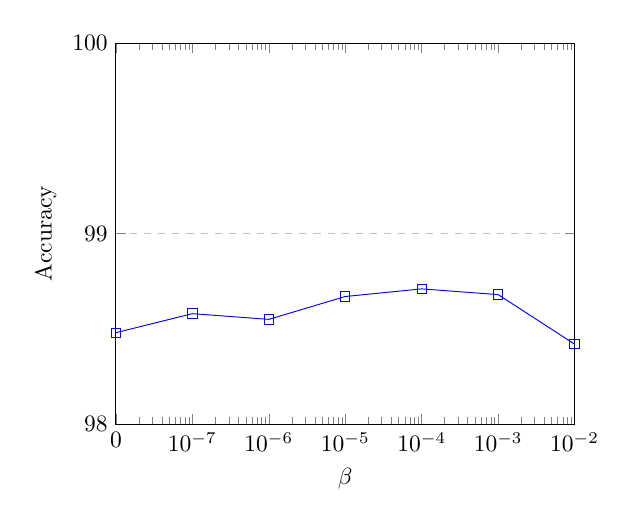
\begin{tikzpicture}[scale = 0.85]
\begin{semilogxaxis}[
    xlabel={$\beta$},
    ylabel={Accuracy},
    xmin=0.00000001, xmax=0.01,
    ymin=98, ymax=100,
    xtick={0.00000001,0.0000001,0.000001,0.00001,0.0001,0.001,0.01},
    xticklabels={0, $10^{-7}$, $10^{-6}$, $10^{-5}$, $10^{-4}$, $10^{-3}$, $10^{-2}$},
    ytick={98, 99, 100},
    ymajorgrids=true,
    grid style=dashed,
]
\addplot[color=blue, mark=square,]
    coordinates {
   (0.00000001,98.48) (0.0000001,98.58)(0.000001,98.55)(0.00001,98.67)(0.0001,98.71)(0.001,98.68)(0.01,98.42)
    }; 
\end{semilogxaxis}
\end{tikzpicture}
\captionof{figure}{Accuracy vs Regularisation Parameter}
\end{center}

Although we don't obtain exactly the same values as in \cite{vib}, our regularisation curve has the same shape, applying the information bottleneck method helps getting a better accuracy on the test set. In our case the best accuracy is achieved for $\beta = 10^{-4}$

\subsection{Behavior when $\beta = 0$}
When $\beta = 0$ we expect the network to become fully deterministic as there is no restriction on the variance of $p_\theta(z|x)$, the lower bound will be maximum when $z = \mu(x)$  that is having $\Sigma$ to be zero. We verify in this experiment that the values of the diagonal covariance matrix tend to zero as the network is trained.

\begin {table}[H]
\begin{center}
\begin{tabular}{ c | c c }
 $\beta$ & $\bar{\Sigma_{ii}}$ \\
 \hline
0 & 0.02\\
1 & 0.99 \\
\end{tabular}
\end{center}
\caption{Average covariance diagonal terms when $\beta$ varies}
\end {table}

After training the network for 200 epochs the average diagonal values of the covariance matrix are indeed close to 0 in the non-regularised case whereas with a very strong regularisation they will be very close to the variational parameters: $r(z) \sim \mathcal{N}(0, I)$

\subsection{Bottleneck size considerations}
In this experiment we change the size of the bottleneck while setting $\beta = 0$, that is we don't explicitly constrain the mutual information between $X$ and $Z$, however we would like to verify that simply reducing the bottleneck size does not have the same effect as setting a non-zero regularisation parameter.

\begin {table}[H]
\begin{center}
\begin{tabular}{ c | c c }
 K & accuracy & loss \\
 \hline
256 & 98.26 & 0.064 \\
128 & 98.14 & 0.065 \\
64 & 98.12& 0.067 \\
32 & 98.09 & 0.066 \\
\end{tabular}
\end{center}
\caption{Performance of the network for different bottleneck sizes}
\end {table}

We see that reducing the bottleneck size does not improve the test accuracy and loss. This is a confirmation that using the mutual information to control the amount of information we let flow from the input to the output is a better quantifier and regulariser.

\subsection{Parametric Marginal}
To improve on the approximation of the marginal $p(z)$ we study the effect of adding two parameter, a mean and a diagonal covariance matrix. We redefined our approximation as

$$r_\psi(x) = \mathcal{N}(\mu_r, \Sigma_r)$$ 

Where $\mu_r$ and $\Sigma_r$ are parameters that can be learned. 

\begin {table}[H]
\begin{center}
\begin{tabular}{ c  c| c c }
 Marginal & $\beta$ & Accuracy & Loss \\
 \hline
Standard &  0 & 98.48 & 0.058 \\
Parametric & 0 & 98.46 & 0.057 \\
Standard &  $10^{-4}$ & 98.71 & 0.053 \\
Parametric & $10^{-4}$ & 98.58 & 0.063 \\
\end{tabular}
\end{center}
\caption{Performance of the network for different bottleneck sizes}
\end {table}

We don't see an improvement of the performance when using the richer approximation. We note that we're still restricting the marginal to be uni-modal and having uncorrelated features.

\section{Many to one}
\subsection{Sequence of MNIST images to single label}
In this experiment we try to predict the label of a first image of a sequence of MNIST images. The network has to "remember" the first image it has seen and associate a label to it. It should learn to discard all the information coming from the rest of the sequence.

\begin{minipage}{0.35\textwidth}
        \centering
\begin{tabular}{ c | c  }
 GRU units & 128 \\
 Bottleneck size & 32 \\
 Sequence length & 5 \\
\end{tabular}
\captionof{figure}{Parameters}
    \end{minipage}\hfill
    \begin{minipage}{0.8\textwidth}
        \centering
\begin{tabular}{ c | c c }
 $\beta$ & accuracy & loss \\
 \hline
0 & 92.90 & 0.290 \\
$10^{-4}$ & 94.05 & 0.273 \\
$10^{-3}$ & 94.55 & 0.293 \\
$10^{-2}$ & 94.35 & 0.271 \\
\end{tabular}
\captionof{figure}{Results}
    \end{minipage}

\begin{center}
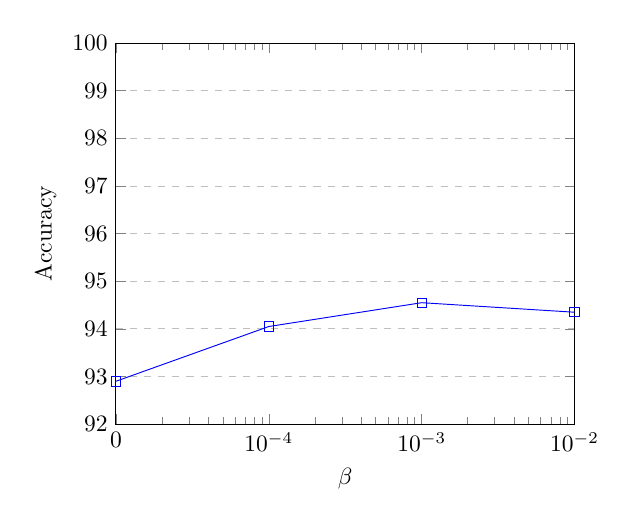
\begin{tikzpicture}[scale = 0.85]
\begin{semilogxaxis}[
    xlabel={$\beta$},
    ylabel={Accuracy},
    xmin=0.00001, xmax=0.01,
    ymin=92, ymax=100,
    xtick={0.00001, 0.0001,0.001,0.01},
    xticklabels={0, $10^{-4}$, $10^{-3}$, $10^{-2}$},
    ytick={92, 93, 94, 95, 96, 97, 98, 99, 100},
    ymajorgrids=true,
    grid style=dashed,
]
\addplot[color=blue, mark=square,]
    coordinates {
   (0.00001,92.90)(0.0001,94.05)(0.001,94.55)(0.01,94.35)
    }; 
\end{semilogxaxis}
\end{tikzpicture}
\captionof{figure}{Accuracy vs Regularisation Parameter}
\end{center}

\subsection{Video of shapes to number of frames seen}

In this experiment we generated videos of different shapes: triangle or squares moving inside a box under the law of gravity. They can freely leave the box on each side but not at the top or bottom and are given an initial momentum. The objective is to measure the number of frames that of each of the shapes spent inside the box. If several instances of the same shape are present we count the number of that shape present for each frame. 

For this problem we use a L2 loss over the normalised outputs instead of the cross entropy since we are trying to predict a real number similarly to a regression problem.

\begin{minipage}{0.35\textwidth}
        \centering
\begin{tabular}{ c | c  }
 Train samples & 400 \\
 Test samples & 100 \\
 Hidden units & 512 \\
 Bottleneck size & 256 \\
 Sequence length & 60 \\
 Frame size & 36 x 36
\end{tabular}
\captionof{figure}{Parameters}
    \end{minipage}\hfill
    \begin{minipage}{0.8\textwidth}
        \centering
\begin{tabular}{ c | c }
 $\beta$ &  loss \\
 \hline
0  & 0.054 \\
$10^{-4}$  & 0.0438 \\
$5.10^{-4}$  & 0.0484 \\
$10^{-3}$  & 0.0510 \\
\end{tabular}
\captionof{figure}{Results}
    \end{minipage}


\section{Sequence to sequence}
\subsection{Sequence of MNIST images to sequence of labels}
In this experiment we give a sequence of images and the objective is to generate the sequence of labels associated to those images in the right order. We separate here the hidden size of the recurrent neural network that goes over the input and the recurrent neural network used to generate the output

\subsubsection{Random order}
In this experiment the images are taken at random with no particular order.

\begin{minipage}{0.35\textwidth}
        \centering
\begin{tabular}{ c | c  }
 Hidden units input & 512 \\
 Hidden units output & 256 \\
 Bottleneck size & 256 \\
 Sequence length & 5 \\
\end{tabular}
\captionof{figure}{Parameters}
    \end{minipage}\hfill
    \begin{minipage}{0.8\textwidth}
        \centering
\begin{tabular}{ c | c c }
 $\beta$ & accuracy & loss \\
 \hline
0  & 90.08 & 0.387 \\
$10^{-5}$  & 90.90 & 0.386 \\
$10^{-4}$  & 92.27 & 0.377 \\
$10^{-3}$  & 90.74 & 0.423 \\
\end{tabular}
\captionof{figure}{Results}
    \end{minipage}

\begin{center}
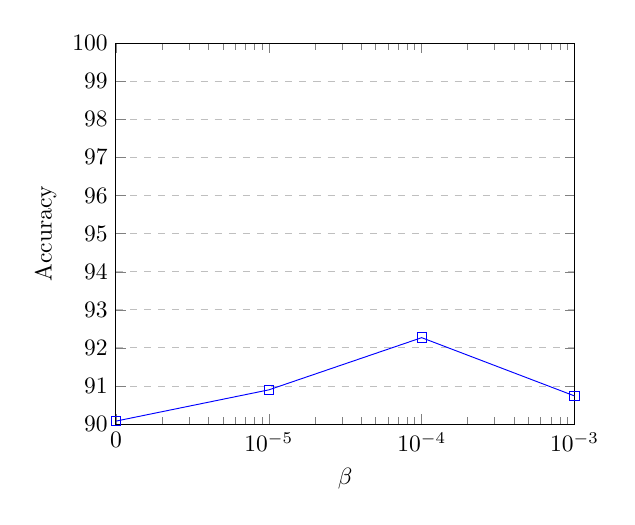
\begin{tikzpicture}[scale = 0.85]
\begin{semilogxaxis}[
    xlabel={$\beta$},
    ylabel={Accuracy},
    xmin=0.000001, xmax=0.001,
    ymin=90, ymax=100,
    xtick={0.000001, 0.00001, 0.0001,0.001},
    xticklabels={0, $10^{-5}$, $10^{-4}$, $10^{-3}$},
    ytick={90, 91, 92, 93, 94, 95, 96, 97, 98, 99, 100},
    ymajorgrids=true,
    grid style=dashed,
]
\addplot[color=blue, mark=square,]
    coordinates {
   (0.000001, 90.08)(0.00001, 90.90)(0.0001, 92.27)(0.001, 90.74)
    }; 
\end{semilogxaxis}
\end{tikzpicture}
\captionof{figure}{Accuracy vs Regularisation Parameter}
\end{center}

As the results indicate, the information bottleneck method was successful in giving better accuracies in the regularised case with on optimium found for $\beta = 10^{-4}$. We will now look in details on some of the learning curves obtained to better understand the process.

\begin{center}
\vspace{1.0cm}
\begin{minipage}{0.5\textwidth}
        \centering
\includegraphics[scale=0.28]{overfit_acc}
    \end{minipage}\hfill
    \begin{minipage}{0.5\textwidth}
        \centering
\includegraphics[scale=0.28]{overfit_loss}
    \end{minipage}
\captionof{figure}{Learning curves of test loss and accuracy for $\beta = 0$ (light green) and $\beta = 10^{-4}$ (dark green) }
\label{fig:overfit}
\vspace{1.0cm}
\end{center}

We see on figure \ref{fig:overfit} that using the information bottleneck regulariser helps preventing overfitting: the test loss stays constant for $\beta$ non zero when it increases for $\beta$ zero after 300 steps. We also note that the accuracy is the regularised case keeps on rising even though the loss is nearly constant. This means that parameters are pushed in the right direction such as to flip images to the right label although overall the loss is not increasing as the learning process might worsen the probability to get a given label without changing the argmax output. Overall our final metric is the accuracy but the loss gives us insights on the learning process.

\subsubsection{Increasing order}
In this experiment the images are ranked with respect to their label so an example of sequence will be 2, 5, 6, 8, 8. This means the recurrent network can used previous digits to improve the guess on the current digit.

\begin{minipage}{0.35\textwidth}
        \centering
\begin{tabular}{ c | c  }
 Hidden units input & 512 \\
 Hidden units output & 256 \\
 Bottleneck size & 256 \\
 Sequence length & 5 \\
\end{tabular}
\captionof{figure}{Parameters}
    \end{minipage}\hfill
    \begin{minipage}{0.8\textwidth}
        \centering
\begin{tabular}{ c | c c }
 $\beta$ & accuracy & loss \\
 \hline
0  & 94.07 & 0.219 \\
$10^{-5}$  & 94.72 & 0.230 \\
$10^{-4}$  & 94.99 & 0.235 \\
$10^{-3}$  & 94.77 & 0.253 \\
\end{tabular}
\captionof{figure}{Results}
    \end{minipage}

\begin{center}
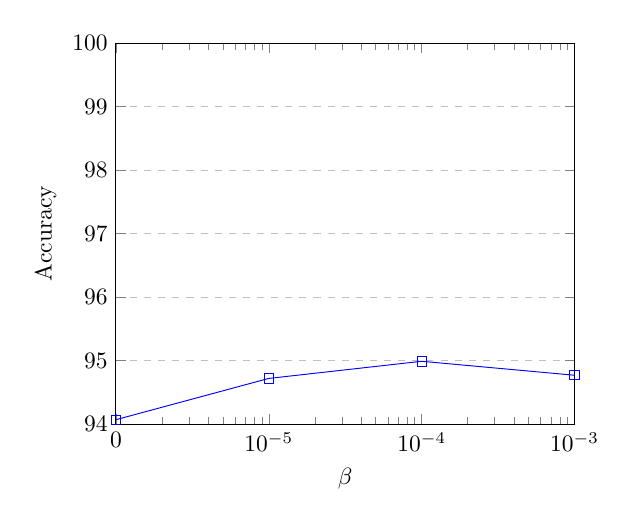
\begin{tikzpicture}[scale = 0.85]
\begin{semilogxaxis}[
    xlabel={$\beta$},
    ylabel={Accuracy},
    xmin=0.000001, xmax=0.001,
    ymin=94, ymax=100,
    xtick={0.000001, 0.00001, 0.0001,0.001,0.01},
    xticklabels={0, $10^{-5}$, $10^{-4}$, $10^{-3}$},
    ytick={94, 95, 96, 97, 98, 99, 100},
    ymajorgrids=true,
    grid style=dashed,
]
\addplot[color=blue, mark=square,]
    coordinates {
   (0.000001, 94.07)(0.00001, 94.72)(0.0001, 94.99)(0.001, 94.77)
    }; 
\end{semilogxaxis}
\end{tikzpicture}
\captionof{figure}{Accuracy vs Regularisation Parameter}
\end{center}

\subsubsection{Using a Convolutional Neural Network}
Instead of to provide as input to the recurrent neural network the raw images (784 pixels) we pass the images trough a convolutional neural network and provide the last fully connected layers as inputs to the RNN. The images do not have a particular order here.

\begin{minipage}{0.35\textwidth}
        \centering
\begin{tabular}{ c | c  }
 Hidden units input & 512 \\
 Hidden units output & 64 \\
 Bottleneck size & 64 \\
 Sequence length & 5 \\
\end{tabular}
\captionof{figure}{Parameters}
    \end{minipage}\hfill
    \begin{minipage}{0.8\textwidth}
        \centering
\begin{tabular}{ c | c c }
 $\beta$ & accuracy & loss \\
 \hline
0  &  99.27  & 0.032 \\
$10^{-5}$  & 99.34 & 0.030  \\
$10^{-4}$  & 99.34 & 0.032  \\
$10^{-3}$  & 99.23 & 0.047  \\
\end{tabular}
\captionof{figure}{Results}
    \end{minipage}

\begin{center}
\begin{tikzpicture}[scale = 0.85]
\begin{semilogxaxis}[
    xlabel={$\beta$},
    ylabel={Accuracy},
    xmin=0.000001, xmax=0.001,
    ymin=99, ymax=100,
    xtick={0.000001, 0.00001, 0.0001,0.001},
    xticklabels={0, $10^{-5}$, $10^{-4}$, $10^{-3}$, $10^{-2}$},
    ytick={99, 100},
    ymajorgrids=true,
    grid style=dashed,
]
\addplot[color=blue, mark=square,]
    coordinates {
   (0.000001, 99.27)(0.00001, 99.34)(0.0001, 99.34)(0.001, 99.23)
    }; 
\end{semilogxaxis}
\end{tikzpicture}
\captionof{figure}{Accuracy vs Regularisation Parameter}
\end{center}

We see here that we greatly outperform the results obtained without using the CNN, this is because the CNN can capture spatial information, each layer learn a higher level representation of the image. Finally the layer that we feed the RNN contain the most relevant information about the label of the image. Passing it through the information bottleneck has less of an effect since the most relevant information has already been extracted by the CNN.

\subsection{Pixel Sequence Prediction}
In this experiment we provide as input a sequence of pixel corresponding to part of the MNIST image. We try to predict the next 15 pixels. At both train and test time, we use the true value of the pixel as inputs to the decoder rather than using the pixels generated by the previous layer. This allows faster and more stable training.

\begin{minipage}{0.35\textwidth}
        \centering
\begin{tabular}{ c | c  }
 Hidden units input & 128 \\
 Hidden units output & 16 \\
 Bottleneck size & 32 \\
 Input sequence length & 60 \\
 Output sequence length & 15 \\
\end{tabular}
\captionof{figure}{Parameters}
    \end{minipage}\hfill
    \begin{minipage}{0.8\textwidth}
        \centering
\begin{tabular}{ c | c c }
 $\beta$ & accuracy & loss \\
 \hline
0  &  97.55  & 0.058 \\
$10^{-5}$  & 97.54 & 0.060  \\
$10^{-4}$  & 97.54 & 0.061  \\
$10^{-3}$  & 97.50 & 0.064  \\
\end{tabular}
\captionof{figure}{Results}
    \end{minipage}
    
    \begin{center}
\begin{tikzpicture}[scale = 0.85]
\begin{semilogxaxis}[
    xlabel={$\beta$},
    ylabel={Accuracy},
    xmin=0.000001, xmax=0.001,
    ymin=97, ymax=100,
    xtick={0.000001, 0.00001, 0.0001,0.001},
    xticklabels={0, $10^{-5}$, $10^{-4}$, $10^{-3}$},
    ytick={97, 98, 99, 100},
    ymajorgrids=true,
    grid style=dashed,
]
\addplot[color=blue, mark=square,]
    coordinates {
   (0.000001, 97.55)(0.00001, 97.54)(0.0001, 97.54)(0.001, 97.50)
    }; 
\end{semilogxaxis}
\end{tikzpicture}
\captionof{figure}{Accuracy vs Regularisation Parameter}
\end{center}

In this case the advantage of the information bottleneck regularisation is not obvious. This might be due to the low dimensionality of the input (binary). In this case having a lower dimensionality bottleneck could help.

\subsection{Translation}
TODO if time allows

%------------------------------------------------------------------------------------------------
\chapter{Conclusion}
\section{Discussion of the results}
As we have seen on the different experiment performed, the information bottleneck method can significantly improve the accuracy of the algorithm in a sequence to sequence as well as in a sequence to label setting. It is especially effective when the inputs of the sequence are high dimensional since the choice of the representation becomes more important. 

We also notice that when dealing with categorical data, the regularisation does not necessarily incuded lower losses but it helped keeping the loss low while the accuracy improved.

\subsection{Attention Models}
State of the art sequence to sequence model for translation and other applications uses attention mechanisms to improve performance. The attention mechanism acts as an external memory to the decoder, at each of the decoder time step, the attention mechanism gives the possibility to go over the inputs that are the most relevant to predict the next output. As the information contained by the input sequence does not have to be contained in the first hidden state of the decoder network, the information bottleneck model does not apply. In fact the only information the "bottleneck" vector needs to contain is the information regarding where to concentrate the attention to predict the first output. Therefore in this dissertation we do not attempt to compare results with attention model.

\subsection{Interpretability}
Using the variational information provides some information in terms of what needs to be encoded such as to predict the output variable. This could be useful in term of interpretability, indeed if it is often difficult to explain the mapping found in the context of neural network. In this case we have vector of fixed size that could be interpreted as features in the same way as other dimensionality reduction techniques.

TODO: more
\section{Limitations}
\subsection{Short running time}
In some of the experiments, we have had to choose an arbitrary number of epochs before we stopped the experiment to keep them under a given computation and time budget even though the performance might still have been increasing. This is not optimal as different degree of regularisation lead to different learning rate. Therefore by stopping early an experiment we might flaw the results.

\subsection{Lack of confidence interval}
For each experiment and each set of the parameters, there should have been a given number of runs done such as to provide a mean and standard deviation of the optimal values. This would have allowed to give us confidence intervals of the values and compare their significance. Given the time and computation budget, we only ran a single run per experiment and set of parameter. Some reassurance comes from the trends obtained by varying the regularisation parameters. Those trend tend to be concave which indicates some coherence in our results. 

\subsection{Tightness of the bound}
To optimise our objective function, we have made two approximations that each adds inaccuracies. To ensure that our optimum is close to the true optimum we would need to do an analysis of the tightness of the bound, possibly using a Markov Chain Monte Carlo sampling until we reach an equilibrium distribution and use those instead of the variational approximation to compare.

\section{Further Work}
TODO: Using CNN to CNN. Compare with other regularisation. Translation. Using normalising flows, etc.

\appendix
%------------------------------------------------------------------------------------------------
\chapter{Appending}
\section{Derivations of the lower bounds}
\subsection{Lower bound of $I(X, Z)$}
\label{appendix:xz}
Given that the KL divergence is necessarily positive we have 

$$ KL\big[p(y|z)|q_\phi(y|z)\big] \geq 0$$ 
\begin{flalign*}
\Rightarrow \quad \int p(y|z) \log \frac{p(y|z)}{q_\phi(y|z)} dy & \geq 0 &\\
\Rightarrow \quad  \int p(y|z) \log p(y|z) dy &\geq \int p(y|z) \log q_\phi(y|z) dy&\\
\Rightarrow \quad \frac{1}{p(z)} \int p(y, z) \log p(y|z) dy &\geq  \frac{1}{p(z)} \int p(y, z) \log q_\phi(y|z) dy&\\
\Rightarrow \quad \int p(y, z) \log p(y|z) dy &\geq  \int p(y, z) \log q_\phi(y|z) dy&\\
\Rightarrow \quad \int p(y, z) \log p(y|z) dy\, dz &\geq  \int p(y, z) \log q_\phi(y|z) dy\, dz&\\
\Rightarrow \quad \int p(y, z) [\log p(y|z) - \log p(y)] dy\, dz & \geq  \int p(y, z) [\log q_\phi(y|z) - \log p(y)] dy\, dz &
\end{flalign*}
And
 \begin{align}
 \Rightarrow I(Z, Y) &\geq  \int p(y, z) \log q_\phi(y|z) dy\, dz + H(Y)\\
	  &=  \int p(x, y, z) \log q_\phi(y|z) dy\, dz\, dx + H(Y)\\
	  &=  \int p(x) p(y|x) p_\theta(z|x) \log q_\phi(y|z) dy\, dz\, dx + H(Y)
\end{align}
\subsection{Lower bound of $I(Z, Y)$}
\label{appendix:zy}
$$ KL[p(z)|r(z)] \geq 0$$
Therefore 
\begin{flalign*}
\int p(z) \log \frac{p(z)}{r(z)} dz &\geq 0 &\\
\Rightarrow \quad \int p(z) \log p(z) dz&\geq \int r(z) \log p(z) dz&\\
\Rightarrow \quad \int p(z, x) \log p(z) dx\, dz &\geq \int r(z, x) \log p(z) dx\, dz&\\
\Rightarrow \quad -\int p(z, x) \log p(z) dx\, dz &\leq - \int r(z, x) \log p(z) dx\, dz&\\
\Rightarrow \quad \int p(z, x) [\log p(z|x) -  \log p(z)]dx\, dz &\leq  \int p(z, x) [\log p(z|x) - \log p(z)]dx\, dz  &\\
\end{flalign*}
And
 \begin{align}
I(X, Z) & \leq  \int p(z, x) \log \frac{p(z|x)}{r(z)} dx\, dz\\
   	  & =  \int p(x, y, z) \log \frac{p(z|x)}{r(z)}dx\, dy\, dz \\
   	  & = \int p(x)p(y|x)p(z|x) \log \frac{p(z|x)}{r(z)}dx\, dy\, dz \\
\end{align}

\section{Other Experiments}
\subsection{Regression}
In this experiment we applied the information bottleneck method to a regression problem: we generated data based on a deterministic function with added noise and try to predict the next 15 points based on a sequence of 60 real numbers.
TODO

\subsection{Binary Pattern}
In this experiment we generated binary data from the following rules:
TODO


\begin{thebibliography}{9} 
\bibitem{barber}
David Barber and Felix Agakov
\textit{The IM Algorithm : A variational approach to Information Maximization}
NIPS 2004
\bibitem{tishby} 
N. Tishby, F.C. Pereira, and W. Biale.
\textit{The information bottleneck method}.
37th annual Allerton Conference on Communication, Control, and Computing, pp. 368-377, 1999.
\bibitem{vib} 
A. A. Alemi, I. Fischer, J. V. Dillon, and K. Murphy
\textit{Deep variational information bottleneck}.
 arXiv:1612.00410, 2016.
 \bibitem{kingma} 
 Diederik P Kingma and Max Welling.
 \textit{Auto-encoding variational Bayes.}
  ICLR, 2014
 \bibitem{gru} 
 Junyoung Chung, Caglar Gulcehre, KyungHyun Cho, Yoshua Bengio.
 \textit{Empirical Evaluation of Gated Recurrent Neural Networks on Sequence Modeling.}
  NIPS, 2014
 \bibitem{graves}
 Graves, Alex.
 \textit{Generating sequences with recurrent neural networks.}
 CoRR, abs/1308.0850, 2013
\bibitem{s2s}
Ilya Sutskever, Oriol Vinyals and Quoc V. Le
\textit{Sequence to Sequence Learning with Neural Networks}
NIPS 2014
\bibitem{attention}
Dzmitry Bahdanau, KyungHyun Cho and Yoshua Bengio
\textit{Neural Machine Translation by Jointly Learning to Align and Translate}
ICLR 2015
\bibitem{vae}
Diederick P. Kingman and Max Welling
\textit{Auto-encoding variational Bayes}
ICLR, 2015
\bibitem{mnist}
Y. LeCun, L. Bottou, Y. Bengio and P. Haffner
\textit{Gradient-based learning applied to document recognition}
IEEE 86 (11), 1998

\bibitem{adam}
D. P. Kingma and J. Ba
\textit{Adam: A method for stochastic optimization.}
 CoRR, abs/1412.6980, 2014
 
\bibitem{vem}
M J. Beal and Z. Ghahramani
\textit{The Variational Bayesian EM Algorithm for Incomplete Data}
Oxford University Press, 2003

\bibitem{draw}
D. Gregor, I. Danihelka, A. Graves, D. Rezende and D. Wierstra
\textit{Draw: A recurrent neural network for image generation}
IICV, 2015
\end{thebibliography}
\end{document}

